% =============================================================================
% Ścieżka Prawa — Dokumentacja Techniczna
% Zwycięski projekt HackNation PL 2025
% Autor: Filip Czerwiński
% =============================================================================
\documentclass[12pt,a4paper]{article}

% === Kodowanie i język polski ===
\usepackage[utf8]{inputenc}
\usepackage[T1]{fontenc}
\usepackage[polish]{babel}
\usepackage{lmodern}

% === Geometria strony ===
\usepackage[margin=2.5cm, top=3cm, bottom=3cm]{geometry}

% === Grafika i kolory ===
\usepackage{graphicx}
\usepackage[table]{xcolor}
\usepackage{float}
\usepackage{wrapfig}

% === Tabele ===
\usepackage{longtable}
\usepackage{booktabs}
\usepackage{tabularx}
\usepackage{multirow}
\usepackage{array}

% === Listingi kodu ===
\usepackage{listings}
\usepackage{inconsolata}

% === Linki i metadane ===
\usepackage[
  colorlinks=true,
  linkcolor=blue!70!black,
  urlcolor=blue!60!black,
  citecolor=blue!70!black,
  bookmarks=true,
  bookmarksopen=true
]{hyperref}

% === Nagłówki i stopki ===
\usepackage{fancyhdr}
\usepackage{lastpage}

% === Enumeracje ===
\usepackage{enumitem}

% === Tikz (diagramy) ===
\usepackage{tikz}
\usetikzlibrary{shapes.geometric, arrows.meta, positioning, calc, fit, backgrounds}

% === Inne ===
\usepackage{tcolorbox}
\tcbuselibrary{skins, breakable}
\usepackage{titlesec}
\usepackage{parskip}

% =============================================================================
% KONFIGURACJA STYLÓW
% =============================================================================

% Kolory
\definecolor{primaryblue}{HTML}{3B82F6}
\definecolor{darkbg}{HTML}{18181B}
\definecolor{codebg}{HTML}{1E1E2E}
\definecolor{codetext}{HTML}{CDD6F4}
\definecolor{codegreen}{HTML}{A6E3A1}
\definecolor{codepurple}{HTML}{CBA6F7}
\definecolor{codeyellow}{HTML}{F9E2AF}
\definecolor{hackgold}{HTML}{D4A017}
\definecolor{accentgreen}{HTML}{22C55E}
\definecolor{accentred}{HTML}{EF4444}
\definecolor{accentpurple}{HTML}{8B5CF6}
\definecolor{sectioncolor}{HTML}{1E3A5F}

% Styl listingów kodu
\lstdefinestyle{typescript}{
  backgroundcolor=\color{codebg},
  basicstyle=\ttfamily\small\color{codetext},
  keywordstyle=\color{codepurple}\bfseries,
  stringstyle=\color{codegreen},
  commentstyle=\color{gray}\itshape,
  numberstyle=\tiny\color{gray},
  numbers=left,
  numbersep=8pt,
  breaklines=true,
  frame=single,
  rulecolor=\color{darkbg},
  tabsize=2,
  showstringspaces=false,
  captionpos=b,
  xleftmargin=12pt,
  framexleftmargin=12pt,
  aboveskip=12pt,
  belowskip=8pt,
  morekeywords={const, let, async, await, export, default, function, return, import, from, interface, type, enum},
}
\lstset{style=typescript}

% Styl SQL
\lstdefinestyle{sql}{
  backgroundcolor=\color{codebg},
  basicstyle=\ttfamily\small\color{codetext},
  keywordstyle=\color{codepurple}\bfseries,
  stringstyle=\color{codegreen},
  commentstyle=\color{gray}\itshape,
  numbers=left,
  numbersep=8pt,
  breaklines=true,
  frame=single,
  rulecolor=\color{darkbg},
  tabsize=2,
  showstringspaces=false,
  morekeywords={CREATE, TABLE, TYPE, ENUM, AS, UUID, TEXT, BOOLEAN, TIMESTAMP, JSONB, DEFAULT, NOT, NULL, PRIMARY, KEY, REFERENCES, WITH, TIME, ZONE, NOW, UNIQUE, CHECK, FOREIGN, INSERT, SELECT, UPDATE, DELETE, FROM, WHERE, AND, OR, ON, CASCADE, SET, IF, EXISTS, POLICY, ENABLE, ROW, LEVEL, SECURITY, USING, auth, uid},
}

% Niestandardowe ramki
\newtcolorbox{infobox}[1][]{
  colback=primaryblue!5,
  colframe=primaryblue!60,
  coltitle=white,
  fonttitle=\bfseries,
  title={#1},
  rounded corners,
  boxrule=0.5pt,
  breakable
}

\newtcolorbox{hackbox}{
  colback=hackgold!8,
  colframe=hackgold,
  coltitle=white,
  fonttitle=\bfseries\large,
  title={$\bigstar$ Zwycięski Projekt HackNation PL 2025},
  rounded corners,
  boxrule=1.5pt,
  arc=4pt,
}

\newtcolorbox{warnbox}[1][]{
  colback=accentred!5,
  colframe=accentred!60,
  coltitle=white,
  fonttitle=\bfseries,
  title={#1},
  rounded corners,
  boxrule=0.5pt,
}

% Styl nagłówków sekcji
\titleformat{\section}
  {\Large\bfseries\color{sectioncolor}}
  {\thesection}{1em}{}[\vspace{-6pt}\textcolor{primaryblue}{\rule{\textwidth}{0.4pt}}]

\titleformat{\subsection}
  {\large\bfseries\color{sectioncolor!80}}
  {\thesubsection}{1em}{}

\titleformat{\subsubsection}
  {\normalsize\bfseries\color{sectioncolor!60}}
  {\thesubsubsection}{1em}{}

% Nagłówek i stopka
\pagestyle{fancy}
\fancyhf{}
\fancyhead[L]{\small\textcolor{gray}{Ścieżka Prawa — Dokumentacja Techniczna}}
\fancyhead[R]{\small\textcolor{gray}{HackNation PL 2025}}
\fancyfoot[C]{\small\textcolor{gray}{Strona \thepage\ z \pageref{LastPage}}}
\fancyfoot[R]{\small\textcolor{gray}{Filip Czerwiński}}
\renewcommand{\headrulewidth}{0.4pt}
\renewcommand{\footrulewidth}{0.2pt}

% Ścieżka do screenshotów
\graphicspath{{../screenshots/}}

% =============================================================================
% DOKUMENT
% =============================================================================
\begin{document}

% === STRONA TYTUŁOWA ===
\begin{titlepage}
\begin{center}

\vspace*{1.5cm}

% Logo / Ikona
\begin{tikzpicture}
  \node[circle, fill=primaryblue, minimum size=2.5cm, inner sep=0pt] (logo) {};
  \node[white, font=\fontsize{36}{36}\selectfont] at (logo) {\textsf{SP}};
\end{tikzpicture}

\vspace{1cm}

{\fontsize{36}{42}\selectfont\bfseries\textcolor{sectioncolor}{Ścieżka Prawa}}

\vspace{0.4cm}

{\Large\textcolor{gray}{Dokumentacja Techniczna Projektu}}

\vspace{1.5cm}

% Baner HackNation
\begin{tikzpicture}
  \node[draw=hackgold, fill=hackgold!10, rounded corners=8pt, line width=1.5pt, 
        inner sep=14pt, font=\large\bfseries] {
    \textcolor{hackgold!80!black}{Zwycięski Projekt — HackNation PL 2025}
  };
\end{tikzpicture}

\vspace{2cm}

{\large\textcolor{gray}{Polski Tracker Legislacyjny}}\\[4pt]
{\large\textcolor{gray}{Next.js 16 + Supabase + AI (Gemini 2.0 Flash)}}

\vspace{2.5cm}

\begin{tabular}{rl}
  \textcolor{gray}{\textbf{Autor:}} & \textbf{Filip Czerwiński} \\[6pt]
  \textcolor{gray}{\textbf{Wersja:}} & 1.1.0 \\[6pt]
  \textcolor{gray}{\textbf{Data:}} & Grudzień 2025 \\[6pt]
  \textcolor{gray}{\textbf{Stos technologiczny:}} & Next.js 16, React 19, TypeScript 5, Supabase \\[6pt]
\end{tabular}

\vfill

{\small\textcolor{gray}{Wersja dokumentacji: 1.0 — Ostatnia aktualizacja: Marzec 2026}}

\end{center}
\end{titlepage}

% === SPIS TREŚCI ===
\tableofcontents
\newpage

% =============================================================================
% SEKCJA 1: WPROWADZENIE
% =============================================================================
\section{Wprowadzenie}

\subsection{O projekcie}

\textbf{Ścieżka Prawa} to nowoczesna platforma webowa do monitorowania procesu legislacyjnego w Polsce. Aplikacja automatycznie synchronizuje dane z oficjalnych API rządowych (Sejm RP, RCL), oferuje analizę AI opartą na modelu Google Gemini 2.0 Flash oraz system spersonalizowanych powiadomień o zmianach w projektach ustaw.

Projekt został stworzony jako odpowiedź na potrzebę zwiększenia przejrzystości procesu tworzenia prawa w Polsce i umożliwienia obywatelom świadomego uczestnictwa w życiu demokratycznym.

\begin{hackbox}
Projekt \textbf{Ścieżka Prawa} zdobył \textbf{pierwsze miejsce} na hackathonie \textbf{HackNation PL 2025} — ogólnopolskim konkursie programistycznym skupionym na rozwiązaniach civic-tech i e-demokracji. Twórcą projektu jest \textbf{Filip Czerwiński}.
\end{hackbox}

\subsection{Główne funkcjonalności}

\begin{itemize}[leftmargin=2em]
  \item \textbf{Śledzenie procesu legislacyjnego} — wizualizacja ścieżki każdego projektu ustawy od wpłynięcia po publikację w Dzienniku Ustaw
  \item \textbf{Synchronizacja z API Sejmu RP} — automatyczne pobieranie danych z \texttt{api.sejm.gov.pl} z 13 statusami ustaw
  \item \textbf{Analiza AI (Gemini 2.0 Flash)} — tłumaczenie na prosty język, analiza skutków, streszczenia, wyjaśnienia terminów prawnych
  \item \textbf{Transmisje na żywo} — detekcja transmisji YouTube kanału @SejmRP\_PL z embedowaniem w aplikacji
  \item \textbf{Konsultacje publiczne} — forum dyskusyjne z wątkami komentarzy i reakcjami
  \item \textbf{Propozycje obywatelskie} — system zgłaszania i głosowania nad poprawkami
  \item \textbf{Ankiety legislacyjne} — tworzenie i wyniki ankiet dotyczących projektów ustaw
  \item \textbf{System powiadomień} — alerty email via Resend API + powiadomienia in-app
  \item \textbf{Wyszukiwarka AI} — inteligentne wyszukiwanie z analizą semantyczną zapytań
  \item \textbf{Panel administracyjny} — zarządzanie użytkownikami, projektami, synchronizacją i ustawieniami
  \item \textbf{Pełna dostępność WCAG} — tryby kontrastu, regulacja rozmiaru czcionki, nawigacja klawiaturą
  \item \textbf{Tryb ciemny/jasny} — pełne wsparcie dark mode z trybem systemowym
\end{itemize}

\subsection{Screenshoty aplikacji}

\begin{figure}[H]
  \centering
  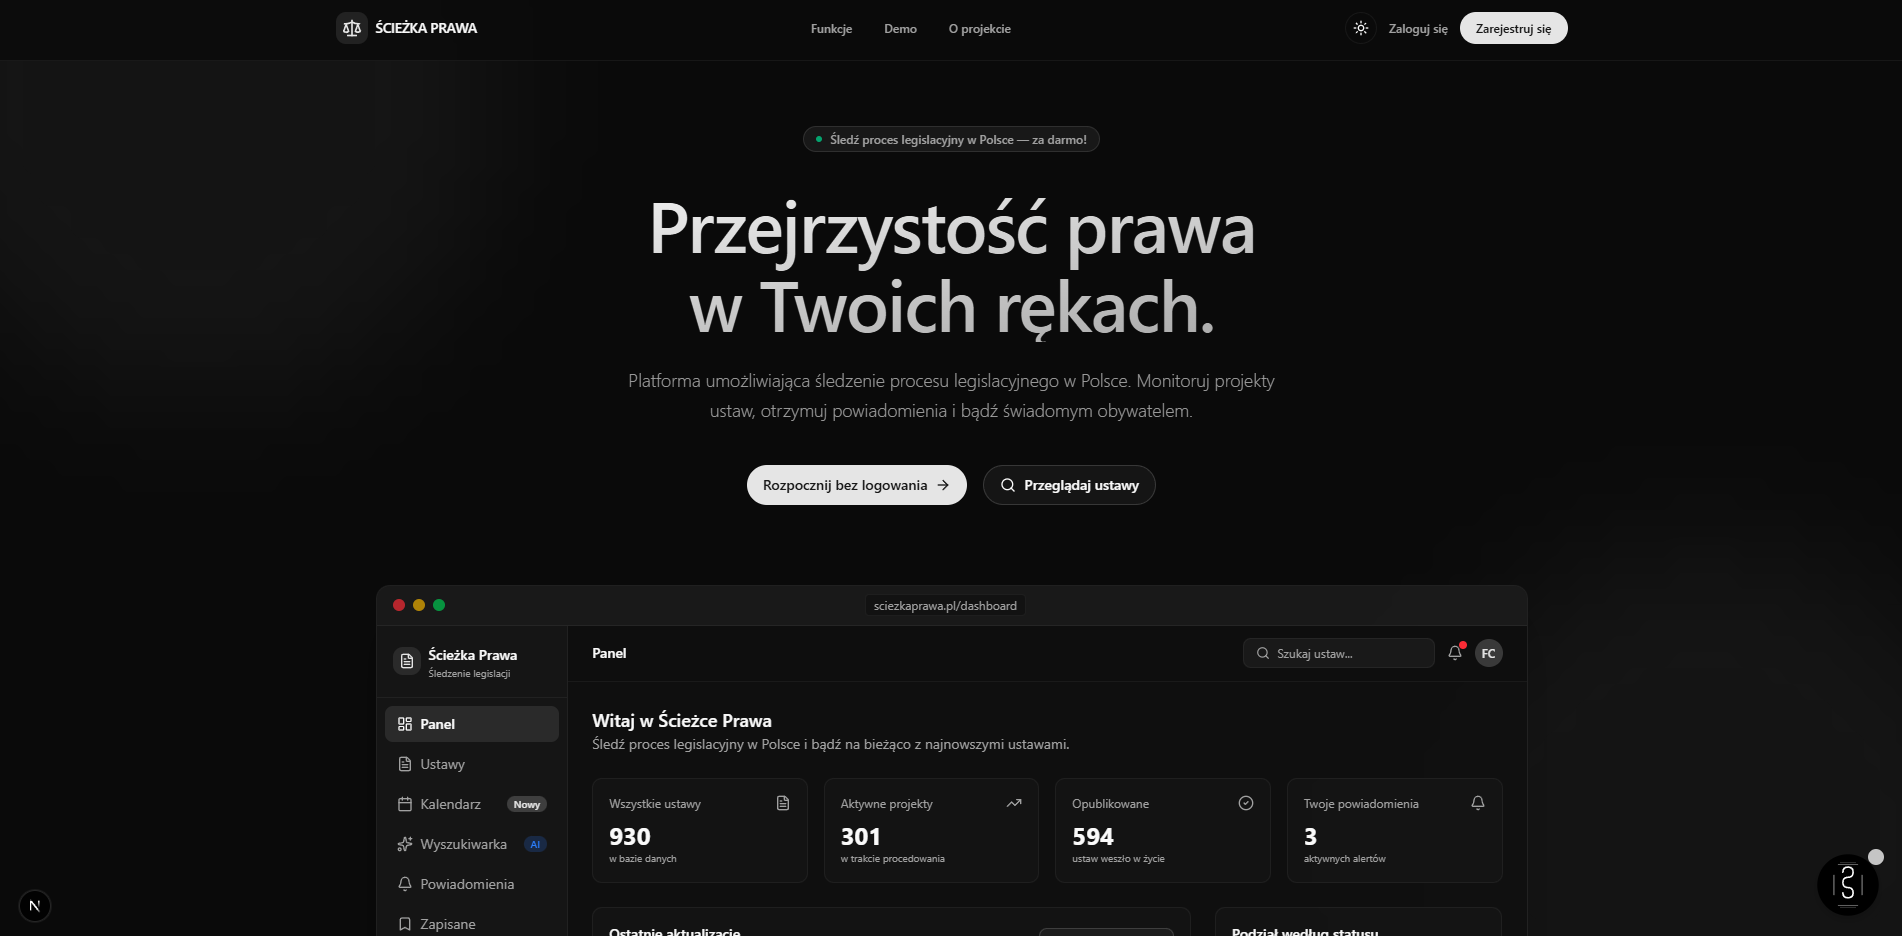
\includegraphics[width=\textwidth]{landing.png}
  \caption{Strona główna (Landing Page) — prezentacja funkcjonalności platformy}
  \label{fig:landing}
\end{figure}

\begin{figure}[H]
  \centering
  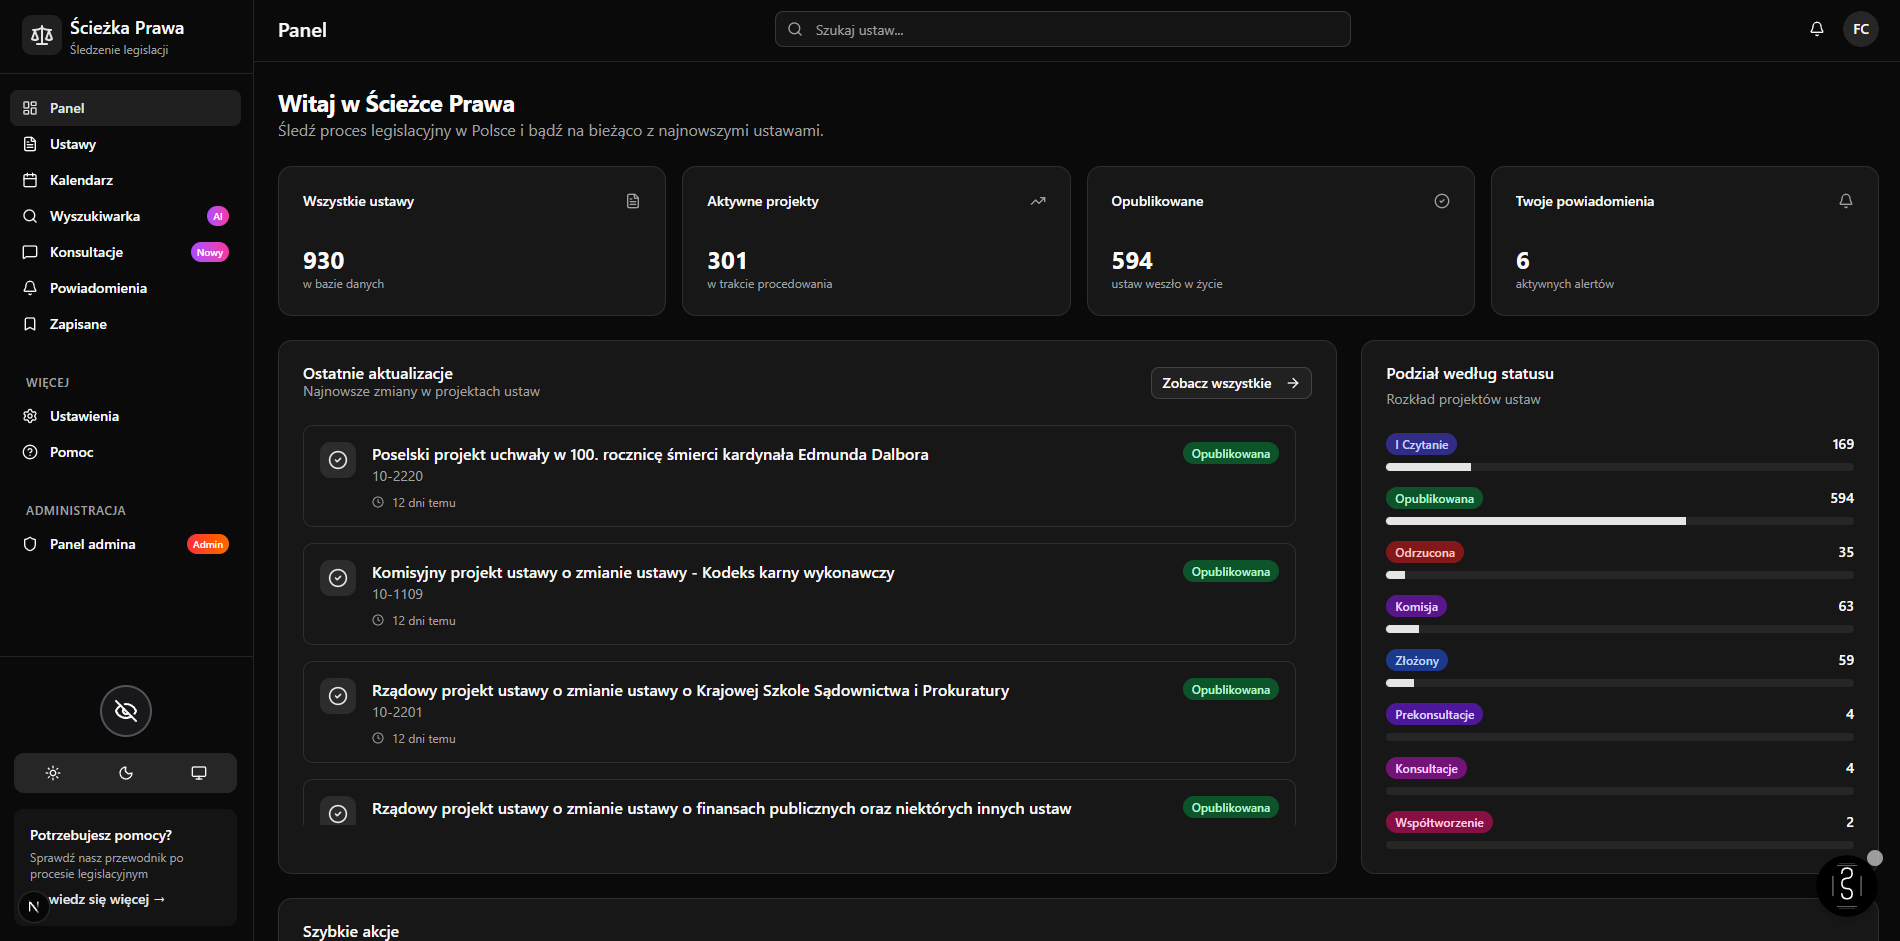
\includegraphics[width=\textwidth]{dashboard.png}
  \caption{Panel główny (Dashboard) — przegląd statystyk, transmisja na żywo i ostatnie aktualizacje}
  \label{fig:dashboard}
\end{figure}

\newpage

% =============================================================================
% SEKCJA 2: ARCHITEKTURA SYSTEMU
% =============================================================================
\section{Architektura systemu}

\subsection{Stos technologiczny}

\begin{table}[H]
\centering
\renewcommand{\arraystretch}{1.4}
\begin{tabularx}{\textwidth}{l l X}
\toprule
\textbf{Warstwa} & \textbf{Technologia} & \textbf{Opis} \\
\midrule
Framework & Next.js 16.0.7 & App Router, Server Components, Turbopack \\
UI & React 19.2.1 & Hooks, Server/Client Components \\
Język & TypeScript 5 & Strict mode, ścieżki aliasów (@/*) \\
Baza danych & Supabase (PostgreSQL) & RLS, Realtime, Auth, Storage \\
Stylowanie & Tailwind CSS 4 & Ciemny motyw, responsywność \\
Komponenty UI & Radix UI + ShadCN & 26 komponentów (Button, Card, Dialog...) \\
AI & Google Gemini 2.0 Flash & 4 tryby analizy tekstu prawnego \\
Email & Resend API & Powiadomienia HTML o zmianach statusu \\
Wykresy & Recharts 3.5.1 & Wizualizacja danych głosowań \\
Ikony & Lucide React & 500+ ikon SVG \\
Daty & date-fns 4.1.0 & Lokalizacja polska (pl) \\
Markdown & marked 17.0.1 & Renderowanie odpowiedzi AI \\
Scraping & Cheerio 1.1.2 & Detekcja YouTube Live \\
PDF & pdf-parse 2.4.5 & Analiza dokumentów OSR \\
Motywy & next-themes 0.4.6 & Light/dark/system \\
Toasty & Sonner 2.0.7 & Powiadomienia UI \\
\bottomrule
\end{tabularx}
\caption{Stos technologiczny projektu}
\label{tab:techstack}
\end{table}

\subsection{Diagram architektury}

\begin{figure}[H]
\centering
\begin{tikzpicture}[
  node distance=1.5cm,
  box/.style={draw, rounded corners=6pt, fill=#1!15, text=#1!90!black, 
              minimum width=3.5cm, minimum height=1cm, font=\small\bfseries,
              text centered, line width=0.5pt, draw=#1!50},
  api/.style={box=primaryblue},
  db/.style={box=accentgreen},
  ui/.style={box=accentpurple},
  ext/.style={box=hackgold},
  arrow/.style={-{Stealth[length=6pt]}, thick, color=gray!70}
]

% External APIs
\node[ext] (sejm) {API Sejmu RP};
\node[ext, right=2cm of sejm] (yt) {YouTube API};
\node[ext, right=2cm of yt] (gemini) {Google Gemini};

% Backend API
\node[api, below=2cm of sejm] (sync) {/api/sync};
\node[api, right=2cm of sync] (ytapi) {/api/youtube-live};
\node[api, right=2cm of ytapi] (aiapi) {/api/ai/*};

% Database
\node[db, below=2cm of ytapi] (supa) {Supabase PostgreSQL};
\node[db, left=1.5cm of supa] (auth) {Supabase Auth};
\node[db, right=1.5cm of supa] (rls) {RLS Policies};

% Frontend
\node[ui, below=2cm of auth] (server) {Server Components};
\node[ui, below=2cm of supa] (client) {Client Components};
\node[ui, below=2cm of rls] (admin) {Panel Admina};

% Arrows - External to API
\draw[arrow] (sejm) -- (sync);
\draw[arrow] (yt) -- (ytapi);
\draw[arrow] (gemini) -- (aiapi);

% Arrows - API to DB
\draw[arrow] (sync) -- (supa);
\draw[arrow] (ytapi) -- (client);
\draw[arrow] (aiapi) -- (client);

% Arrows - DB to Frontend
\draw[arrow] (supa) -- (server);
\draw[arrow] (supa) -- (client);
\draw[arrow] (auth) -- (server);
\draw[arrow] (rls) -- (admin);

% Email
\node[ext, below=1.5cm of client] (resend) {Resend (Email)};
\draw[arrow, dashed] (client) -- (resend);

% Labels
\node[above=0.3cm of sejm, font=\footnotesize\color{gray}] {Zewnętrzne API};
\node[above=0.3cm of sync, font=\footnotesize\color{gray}, xshift=2cm] {API Routes (Next.js)};
\node[above=0.3cm of supa, font=\footnotesize\color{gray}, xshift=-1cm] {Baza danych};
\node[above=0.3cm of client, font=\footnotesize\color{gray}] {Frontend};

\end{tikzpicture}
\caption{Diagram architektury systemu Ścieżka Prawa}
\label{fig:architecture}
\end{figure}

\subsection{Przepływ danych}

\begin{enumerate}[leftmargin=2em]
  \item \textbf{Sejm API → Sync → Supabase}: Endpoint \texttt{/api/admin/sync} pobiera dane z \texttt{api.sejm.gov.pl}, mapuje statusy na podstawie pól \texttt{ELI}/\texttt{passed} i zapisuje do tabel \texttt{bills} + \texttt{bill\_events}
  \item \textbf{Server Components → Supabase → Klient}: Strony używają serwerowej funkcji \texttt{createClient()} do pobierania danych
  \item \textbf{Client Components → Supabase}: Komponenty klienckie korzystają z przeglądarowej wersji klienta do autentykacji i profilów
  \item \textbf{AI Pipeline}: Tekst ustawy → Google Gemini 2.0 Flash → Markdown → Renderowanie w UI
\end{enumerate}

\newpage

% =============================================================================
% SEKCJA 3: STRUKTURA PROJEKTU
% =============================================================================
\section{Struktura projektu}

\subsection{Organizacja katalogów}

\begin{lstlisting}[style=typescript, title=Struktura katalogów projektu]
sciezka-prawa/
  src/
    app/                    # App Router (Next.js 16)
      layout.tsx            # Root layout z ThemeProvider
      page.tsx              # Landing page (strona glowna)
      globals.css           # Style globalne + Tailwind
      admin/                # Panel administracyjny (4 podstrony)
      alerts/               # Zarzadzanie alertami uzytkownika
      api/                  # API Routes (34 endpointy)
        admin/              # Endpointy admina (sync, users, settings)
        ai/                 # AI endpoints (chat, simple-language)
        alerts/             # CRUD alertow
        calendar/           # Kalendarz legislacyjny
        consultation-comments/  # Forum konsultacji
        notifications/      # System powiadomien (8 endpointow)
        proposals/          # Propozycje obywatelskie
        search/             # Wyszukiwarka AI
        surveys/            # Ankiety legislacyjne
        votings/            # Wyniki glosowan
        youtube-live/       # Detekcja transmisji
      auth/                 # Autentykacja (login, callback)
      bills/                # Projekty ustaw (lista + szczegoly)
      calendar/             # Kalendarz posiedzen
      consultations/        # Konsultacje publiczne
      dashboard/            # Panel glowny
      search/               # Wyszukiwarka
      ...
    components/
      ui/                   # 26 komponentow ShadCN (Button, Card...)
      layout/               # Sidebar, Header, MobileNav, DashboardLayout
      bills/                # Komponenty ustaw (15+ komponentow)
      accessibility/        # Tryby kontrastu, rozmiary czcionek
      landing/              # Komponenty strony glownej
      notifications/        # Centrum powiadomien
      providers/            # ThemeProvider, AccessibilityProvider
    lib/
      supabase/             # Klienty Supabase (server + client)
      api/                  # Klient API Sejmu
      admin/                # System uprawnien
      ai/                   # Baza wiedzy AI (RAG)
      email/                # Szablony email (Resend)
    types/
      supabase.ts           # Typy TypeScript (generowane)
  supabase/
    schema.sql              # Pelny schemat bazy danych
  docs/                     # Dokumentacja
\end{lstlisting}

\subsection{Wzorzec Server/Client Component}

Aplikacja stosuje konsekwentny wzorzec rozdzielenia komponentów serwera i klienta:

\begin{lstlisting}[style=typescript, title=Wzorzec Server Component + Client Content]
// src/app/bills/page.tsx (Server Component)
export default async function BillsPage({ searchParams }: Props) {
  const supabase = await createClient()
  const { data: bills } = await supabase.from('bills').select('*')
  return (
    <DashboardLayout user={user}>
      <BillsContent bills={bills} />
    </DashboardLayout>
  )
}

// src/app/bills/bills-content.tsx (Client Component)
'use client'
export function BillsContent({ bills }: Props) {
  // Interaktywna logika UI: filtry, sortowanie, paginacja
}
\end{lstlisting}

\newpage

% =============================================================================
% SEKCJA 4: BAZA DANYCH
% =============================================================================
\section{Baza danych}

\subsection{Schemat bazy danych}

System korzysta z \textbf{Supabase} (PostgreSQL) z włączonym \textbf{Row-Level Security (RLS)} na wszystkich tabelach.

\subsubsection{Typy wyliczeniowe (ENUM)}

\begin{lstlisting}[style=sql, title=Typy ENUM w PostgreSQL]
CREATE TYPE bill_status AS ENUM (
  'co_creation',      -- Wspoltworzenie obywatelskie
  'preconsultation',  -- Prekonsultacja
  'consultation',     -- Konsultacje publiczne (RCL)
  'draft',            -- Projekt wstepny
  'submitted',        -- Wplyniecie do Sejmu
  'first_reading',    -- I Czytanie
  'committee',        -- Prace komisji
  'second_reading',   -- II Czytanie
  'third_reading',    -- III Czytanie i glosowanie
  'senate',           -- Senat
  'presidential',     -- Podpis Prezydenta
  'published',        -- Opublikowana (Dz.U.)
  'rejected'          -- Odrzucona
);

CREATE TYPE user_role AS ENUM (
  'user',         -- Uzytkownik standardowy
  'moderator',    -- Moderator (edycja/ukrywanie)
  'admin',        -- Administrator
  'super_admin'   -- Super administrator
);

CREATE TYPE reaction_type AS ENUM (
  'like', 'support', 'insightful'
);
\end{lstlisting}

\subsubsection{Tabela: bills (Projekty ustaw)}

\begin{table}[H]
\centering
\renewcommand{\arraystretch}{1.3}
\footnotesize
\begin{tabularx}{\textwidth}{l l l X}
\toprule
\textbf{Kolumna} & \textbf{Typ} & \textbf{Nullable} & \textbf{Opis} \\
\midrule
id & UUID & PK & Identyfikator (gen\_random\_uuid) \\
sejm\_id & TEXT & UNIQUE & ID z API Sejmu \\
title & TEXT & NOT NULL & Tytuł projektu \\
description & TEXT & & Opis projektu \\
status & bill\_status & DEFAULT draft & Status legislacyjny (13 wartości) \\
ministry & TEXT & & Ministerstwo odpowiedzialne \\
submission\_date & TIMESTAMP & & Data wpłynięcia \\
last\_updated & TIMESTAMP & & Ostatnia aktualizacja \\
external\_url & TEXT & & Link do Sejm.gov.pl \\
document\_type & TEXT & & Typ dokumentu \\
submitter\_type & TEXT & & Typ wnioskodawcy \\
category & TEXT & & Kategoria tematyczna \\
term & INTEGER & & Kadencja (np. 10) \\
tags & TEXT[] & & Tagi (tablica) \\
submission\_year & INTEGER & & Rok wpłynięcia \\
is\_hidden & BOOLEAN & DEFAULT false & Czy ukryty przez admina \\
rcl\_id & TEXT & & ID z systemu RCL \\
consultation\_start\_date & TIMESTAMP & & Początek konsultacji \\
consultation\_end\_date & TIMESTAMP & & Koniec konsultacji \\
consultation\_url & TEXT & & Link do konsultacji \\
impact\_assessment\_url & TEXT & & Link do OSR \\
simple\_language\_summary & TEXT & & Streszczenie AI \\
created\_at & TIMESTAMP & DEFAULT now() & Data utworzenia \\
updated\_at & TIMESTAMP & DEFAULT now() & Data modyfikacji \\
\bottomrule
\end{tabularx}
\caption{Schemat tabeli \texttt{bills}}
\end{table}

\subsubsection{Tabela: bill\_events (Zdarzenia legislacyjne)}

\begin{table}[H]
\centering
\renewcommand{\arraystretch}{1.3}
\footnotesize
\begin{tabularx}{\textwidth}{l l l X}
\toprule
\textbf{Kolumna} & \textbf{Typ} & \textbf{Nullable} & \textbf{Opis} \\
\midrule
id & UUID & PK & Identyfikator \\
bill\_id & UUID & FK → bills & Powiązanie z projektem \\
event\_type & TEXT & NOT NULL & Typ zdarzenia \\
event\_date & TIMESTAMP & & Data zdarzenia \\
description & TEXT & & Opis etapu \\
details & JSONB & & Szczegóły (elastyczne dane) \\
created\_at & TIMESTAMP & DEFAULT now() & \\
\bottomrule
\end{tabularx}
\caption{Schemat tabeli \texttt{bill\_events}}
\end{table}

\subsubsection{Tabela: profiles (Profile użytkowników)}

\begin{table}[H]
\centering
\renewcommand{\arraystretch}{1.3}
\footnotesize
\begin{tabularx}{\textwidth}{l l l X}
\toprule
\textbf{Kolumna} & \textbf{Typ} & \textbf{Nullable} & \textbf{Opis} \\
\midrule
id & UUID & PK, FK → auth.users & Identyfikator z Supabase Auth \\
email & TEXT & UNIQUE & Adres email \\
full\_name & TEXT & & Pełna nazwa \\
avatar\_url & TEXT & & URL awatara \\
role & user\_role & DEFAULT user & Rola w systemie \\
is\_active & BOOLEAN & DEFAULT true & Czy aktywny (blokada) \\
last\_login & TIMESTAMP & & Ostatnie logowanie \\
created\_at & TIMESTAMP & DEFAULT now() & \\
updated\_at & TIMESTAMP & DEFAULT now() & \\
\bottomrule
\end{tabularx}
\caption{Schemat tabeli \texttt{profiles}}
\end{table}

\subsubsection{Dodatkowe tabele}

\begin{table}[H]
\centering
\renewcommand{\arraystretch}{1.3}
\footnotesize
\begin{tabularx}{\textwidth}{l X}
\toprule
\textbf{Tabela} & \textbf{Opis} \\
\midrule
user\_alerts & Subskrypcje użytkowników na zmiany w projektach (user\_id, bill\_id, notify\_email, notify\_push) \\
saved\_searches & Zapisane wyszukiwania z filtrami (name, query, filters JSONB) \\
admin\_logs & Dziennik aktywności administratorów (action, target\_type, target\_id, details, ip\_address) \\
system\_settings & Ustawienia systemowe (key-value z JSONB i opisem) \\
consultation\_comments & Komentarze konsultacyjne z wątkami (parent\_comment\_id, content, is\_edited) \\
consultation\_comment\_reactions & Reakcje na komentarze (like, support, insightful) \\
notifications & Powiadomienia in-app (type, title, message, is\_read, link) \\
\bottomrule
\end{tabularx}
\caption{Dodatkowe tabele w systemie}
\end{table}

\subsection{Polityki Row-Level Security (RLS)}

\begin{lstlisting}[style=sql, title=Kluczowe polityki RLS]
-- Bills: Wszyscy czytaja, moderatorzy edytuja
ALTER TABLE bills ENABLE ROW LEVEL SECURITY;
CREATE POLICY "bills_select" ON bills FOR SELECT
  USING (true);  -- Publiczny dostep do odczytu

-- User Alerts: Kazdy zarzadza wlasnymi
CREATE POLICY "alerts_own" ON user_alerts
  FOR ALL USING (auth.uid() = user_id);

-- Profiles: Publiczny odczyt, prywatny zapis
CREATE POLICY "profiles_read" ON profiles FOR SELECT
  USING (true);
CREATE POLICY "profiles_update" ON profiles FOR UPDATE
  USING (auth.uid() = id);

-- Admin: Service Role Key omija RLS
-- (uzywane do synchronizacji i operacji admina)
\end{lstlisting}

\newpage

\begin{figure}[H]
  \centering
  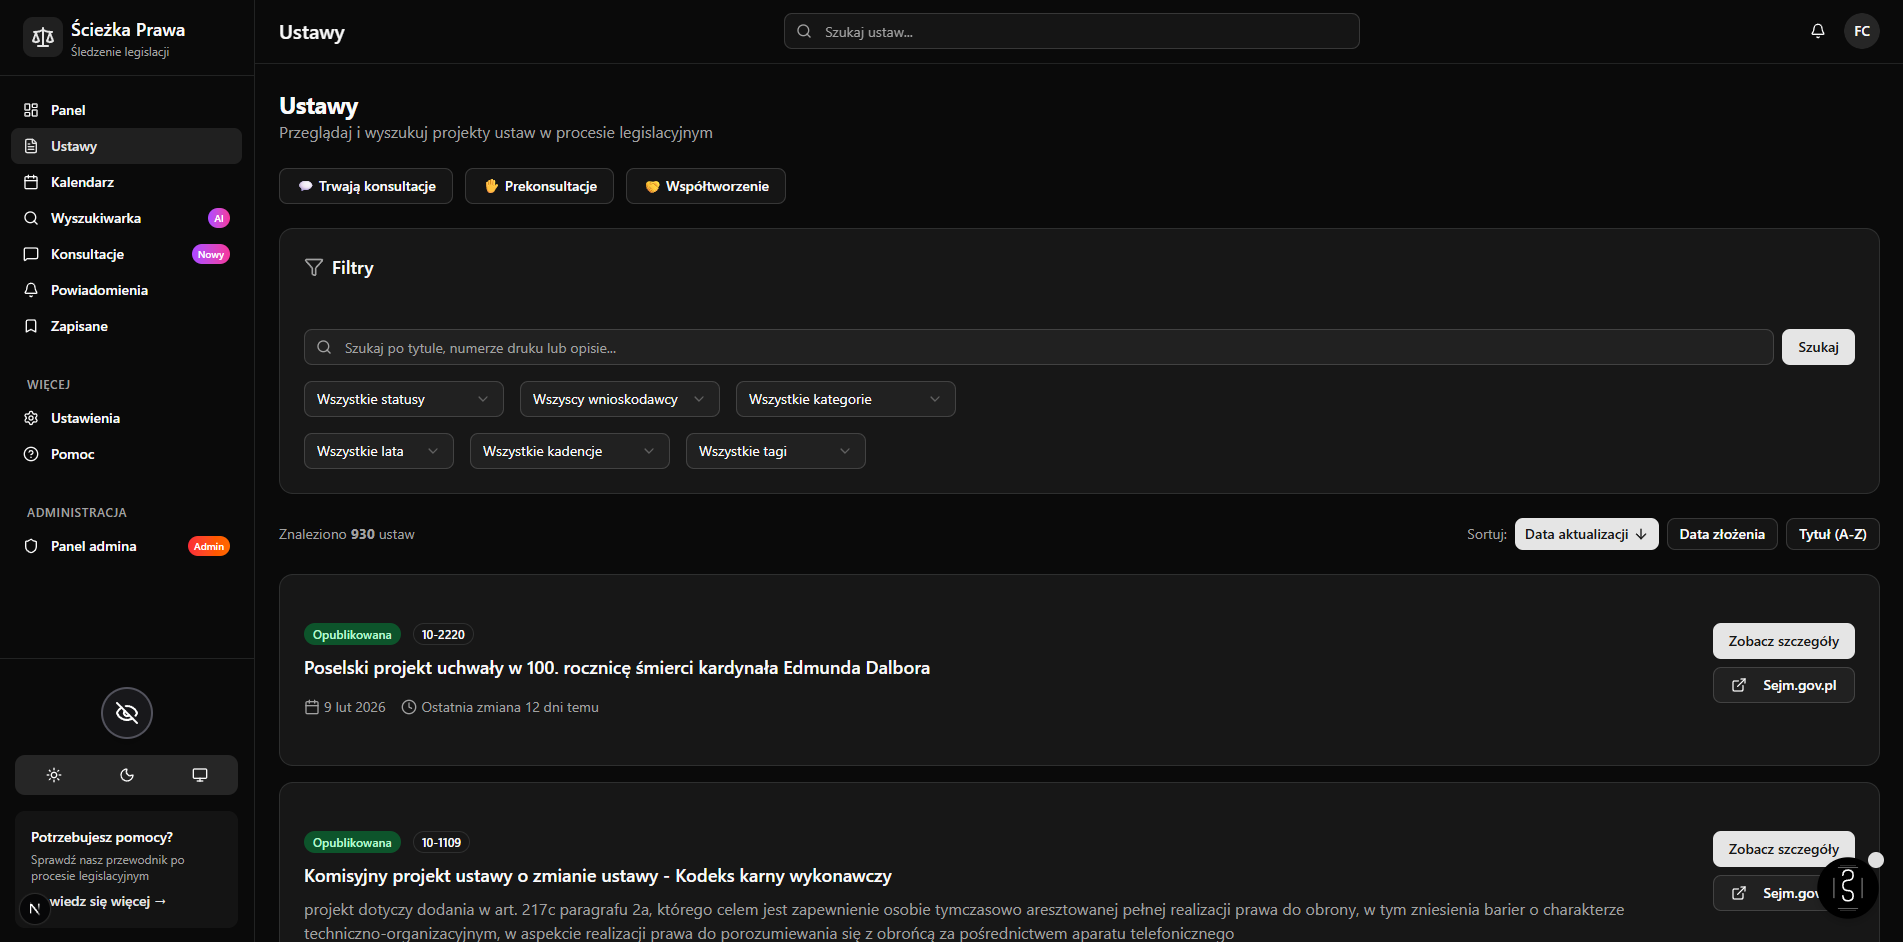
\includegraphics[width=\textwidth]{bills.png}
  \caption{Lista projektów ustaw z zaawansowanymi filtrami i sortowaniem}
  \label{fig:bills}
\end{figure}

% =============================================================================
% SEKCJA 5: API
% =============================================================================
\section{Integracje API}

\subsection{API Sejmu RP}

Główne źródło danych legislacyjnych. Aplikacja korzysta z publicznego API \texttt{api.sejm.gov.pl} dla X kadencji Sejmu.

\begin{table}[H]
\centering
\renewcommand{\arraystretch}{1.3}
\begin{tabularx}{\textwidth}{l l X}
\toprule
\textbf{Endpoint} & \textbf{Metoda} & \textbf{Opis} \\
\midrule
\texttt{/sejm/term10/processes} & GET & Lista wszystkich procesów legislacyjnych \\
\texttt{/sejm/term10/processes/\{nr\}} & GET & Szczegóły procesu ze stagami \\
\texttt{/sejm/term10/committees/\{code\}/sittings} & GET & Posiedzenia komisji z URL video \\
\bottomrule
\end{tabularx}
\caption{Endpointy API Sejmu RP}
\end{table}

\subsubsection{Algorytm mapowania statusów}

Logika określania statusu projektu ustawy (\texttt{src/lib/api/sejm.ts}):

\begin{lstlisting}[style=typescript, title=Algorytm getStatusFromStages()]
function getStatusFromStages(process): BillStatus {
  // Priorytet 1: Publikacja (ELI lub passed=true)
  if (process.ELI || process.passed) return 'published'
  
  // Priorytet 2: Odrzucenie
  if (title.includes('odrzucony')) return 'rejected'
  
  // Priorytet 3: Analiza ostatniego etapu
  const lastStage = stages[stages.length - 1].stageName.toLowerCase()
  
  if (lastStage.includes('ogłoszenie'))    return 'published'
  if (lastStage.includes('prezydent'))     return 'presidential'
  if (lastStage.includes('senat'))         return 'senate'
  if (lastStage.includes('iii czytanie'))  return 'third_reading'
  if (lastStage.includes('ii czytanie'))   return 'second_reading'
  if (lastStage.includes('komisj'))        return 'committee'
  if (lastStage.includes('i czytanie'))    return 'first_reading'
  if (lastStage.includes('skierowanie'))   return 'first_reading'
  
  return 'submitted'  // Domyslny status
}
\end{lstlisting}

\subsection{Google Gemini 2.0 Flash (AI)}

Integracja z modelem \texttt{gemini-2.0-flash} do analizy tekstu prawnego.

\begin{table}[H]
\centering
\renewcommand{\arraystretch}{1.3}
\begin{tabularx}{\textwidth}{l l X}
\toprule
\textbf{Tryb} & \textbf{Endpoint} & \textbf{Opis} \\
\midrule
\texttt{simple} & POST /api/ai/simple-language & Tłumaczenie na prosty język polski \\
\texttt{impact} & POST /api/ai/simple-language & Analiza skutków (obywatele, firmy, budżet) \\
\texttt{summary} & POST /api/ai/simple-language & Streszczenie w 3-5 zdaniach \\
\texttt{explain} & POST /api/ai/simple-language & Wyjaśnienie terminologii prawnej \\
\texttt{chat} & POST /api/ai/chat & Asystent konwersacyjny z bazą wiedzy \\
\texttt{search} & POST /api/search/ai & Inteligentna analiza zapytań wyszukiwania \\
\bottomrule
\end{tabularx}
\caption{Tryby AI w systemie}
\end{table}

\begin{infobox}[Limity Free Tier Gemini API]
  \begin{itemize}[leftmargin=1em]
    \item 15 zapytań na minutę
    \item 1500 zapytań dziennie
    \item 1 000 000 tokenów dziennie
    \item Cachowanie odpowiedzi w localStorage (24h)
  \end{itemize}
\end{infobox}

\subsection{YouTube Live Detection}

Detekcja transmisji na żywo z kanału Sejmu RP bez klucza API:

\begin{lstlisting}[style=typescript, title=Mechanizm detekcji YouTube Live]
// GET /api/youtube-live
// Scraping strony youtube.com/@SejmRP_PL/live
// Wyszukiwanie videoId za pomoca regex
// Cache: 60s revalidation

Response: {
  isLive: boolean,
  videoId: string | null,
  title: string | null,
  channelUrl: "https://www.youtube.com/@SejmRP_PL"
}
\end{lstlisting}

\subsection{Resend API (Email)}

System powiadomień email z szablonami HTML:

\begin{itemize}[leftmargin=2em]
  \item \textbf{Zmiana statusu} — HTML email z badge statusu i linkiem do projektu
  \item \textbf{Raport zbiorczy} — Digest email (dzienny/tygodniowy) z listą zmian
  \item \textbf{Powiadomienie powitalne} — Email po rejestracji nowego użytkownika
\end{itemize}

\newpage

\begin{figure}[H]
  \centering
  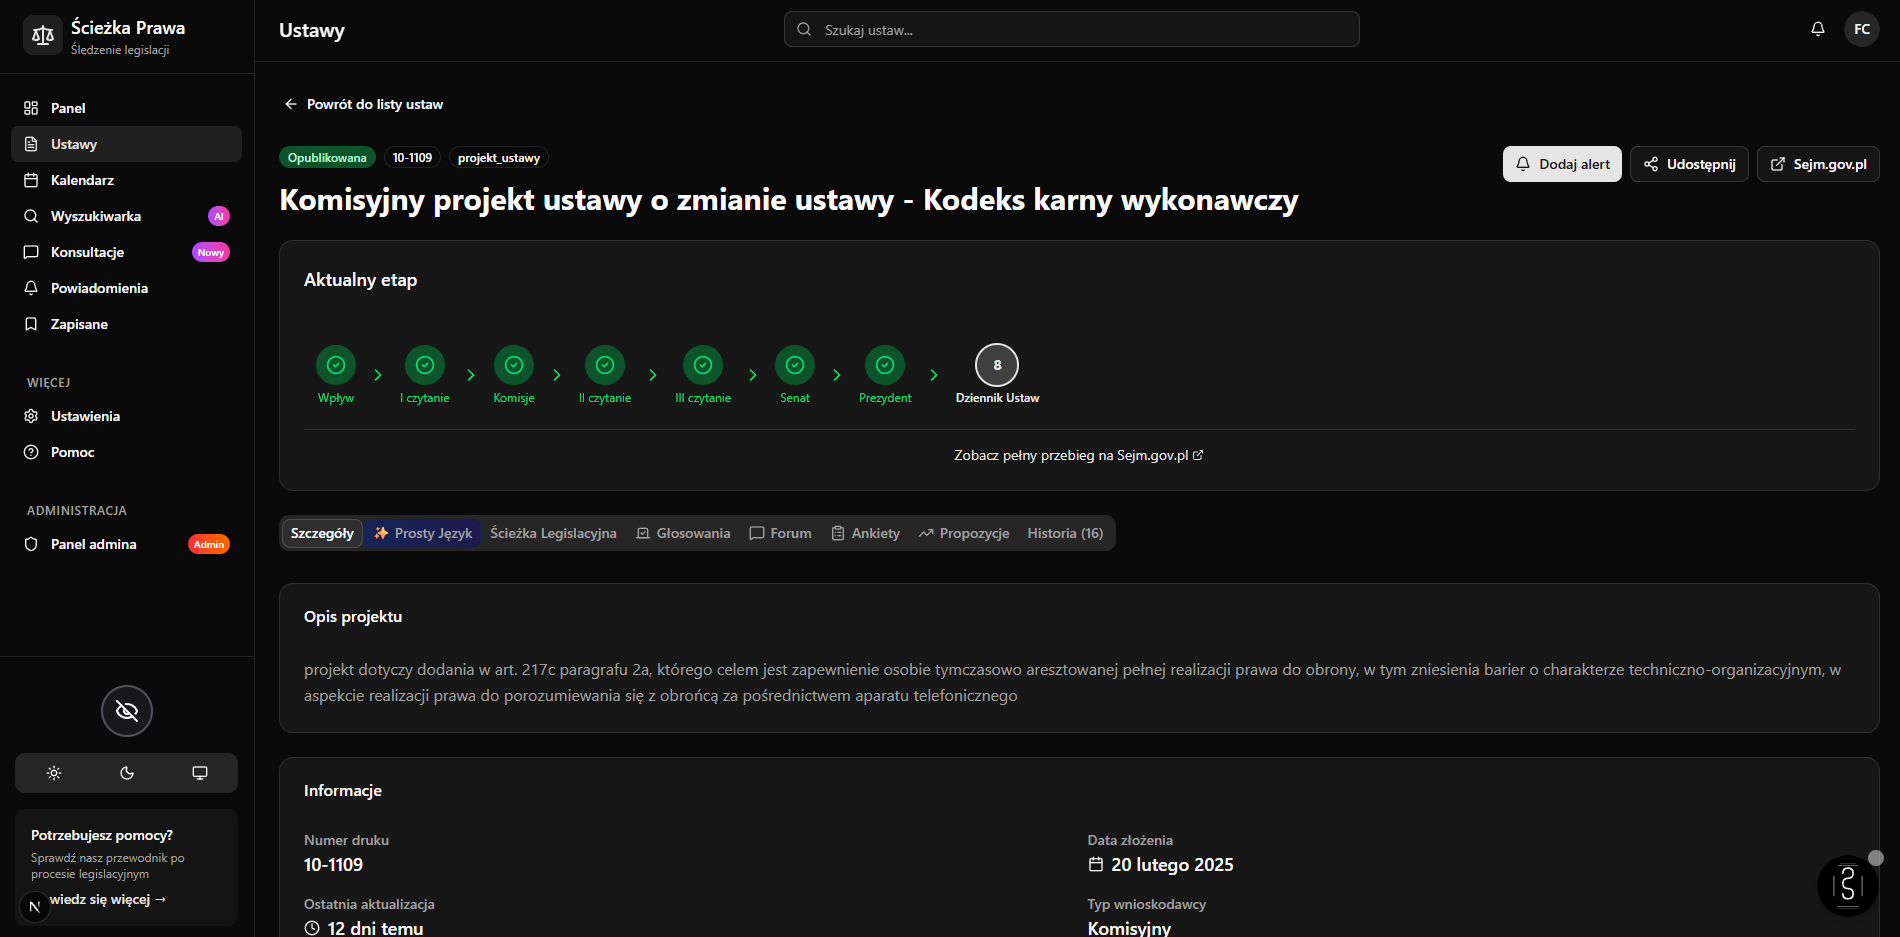
\includegraphics[width=\textwidth]{bill-detail.png}
  \caption{Widok szczegółów projektu ustawy z osią czasu legislacyjną i analizą AI}
  \label{fig:billdetail}
\end{figure}

% =============================================================================
% SEKCJA 6: ENDPOINTY API APLIKACJI
% =============================================================================
\section{Endpointy API aplikacji}

System udostępnia \textbf{34 endpointy} REST API zorganizowane w następujące grupy:

\subsection{Endpointy publiczne i użytkownika}

\begin{table}[H]
\centering
\renewcommand{\arraystretch}{1.3}
\footnotesize
\begin{tabularx}{\textwidth}{l l l X}
\toprule
\textbf{Ścieżka} & \textbf{Metody} & \textbf{Auth} & \textbf{Opis} \\
\midrule
/api/alerts & GET, POST, DELETE & Tak & CRUD alertów użytkownika \\
/api/calendar & GET & Nie & Zdarzenia Sejmu/Senatu z datami \\
/api/consultation-comments & GET, POST, PATCH, DEL & Tak* & Forum komentarzy (wątki) \\
/api/proposals & GET, POST, PATCH, DEL & Tak* & Propozycje poprawek \\
/api/proposals/vote & POST & Tak & Głosowanie na propozycje \\
/api/surveys & GET, POST & Tak & Ankiety legislacyjne \\
/api/surveys/respond & POST & Tak & Odpowiedzi na ankiety \\
/api/search/ai & POST & Nie & AI analiza wyszukiwania \\
/api/ai/simple-language & POST & Nie & Tłumaczenie AI (4 tryby) \\
/api/ai/chat & POST & Nie & Asystent AI konwersacyjny \\
/api/youtube-live & GET & Nie & Status transmisji YouTube \\
/api/votings/\{nr\} & GET & Nie & Wyniki głosowań w Sejmie \\
/api/notifications & GET, PATCH, DEL & Tak & Zarządzanie powiadomieniami \\
/api/account/delete & DELETE & Tak & Usunięcie konta \\
\bottomrule
\end{tabularx}
\caption{Endpointy publiczne i użytkownika (* — GET publiczny, modyfikacje wymagają auth)}
\end{table}

\subsection{Endpointy administracyjne}

\begin{table}[H]
\centering
\renewcommand{\arraystretch}{1.3}
\footnotesize
\begin{tabularx}{\textwidth}{l l l X}
\toprule
\textbf{Ścieżka} & \textbf{Metody} & \textbf{Rola} & \textbf{Opis} \\
\midrule
/api/admin/sync & POST & admin+ & Synchronizacja z API Sejmu \\
/api/admin/sync/\{nr\} & POST & admin+ & Sync konkretnego projektu \\
/api/admin/sync-rcl & POST & admin+ & Synchronizacja z RCL \\
/api/admin/sync-rcl-enhanced & POST & admin+ & Rozszerzona sync RCL \\
/api/admin/users & GET, PATCH & admin+ & Zarządzanie użytkownikami \\
/api/admin/bills/\{id\} & PATCH, DELETE & mod+ & Edycja/ukrywanie projektów \\
/api/admin/settings & GET, PUT & admin+ & Ustawienia systemowe \\
/api/admin/logs & GET & admin+ & Dziennik aktywności \\
/api/admin/parse-osr & POST & admin+ & Parsowanie OSR (PDF) \\
/api/notifications/send & POST & system & Wysyłka powiadomień \\
/api/notifications/process & POST & system & Przetwarzanie kolejki \\
\bottomrule
\end{tabularx}
\caption{Endpointy administracyjne (mod+ = moderator i wyżej, admin+ = admin i wyżej)}
\end{table}

\newpage

% =============================================================================
% SEKCJA 7: SYSTEM UPRAWNIEŃ
% =============================================================================
\section{System uprawnień i bezpieczeństwo}

\subsection{Hierarchia ról}

\begin{figure}[H]
\centering
\begin{tikzpicture}[
  role/.style={draw, rounded corners=4pt, minimum width=3cm, minimum height=0.9cm, 
               font=\small\bfseries, text centered},
  arrow/.style={-{Stealth[length=5pt]}, thick, color=gray!60}
]
  \node[role, fill=hackgold!20, draw=hackgold!60] (sa) at (0, 3) {super\_admin};
  \node[role, fill=accentred!15, draw=accentred!50] (a) at (0, 1.8) {admin};
  \node[role, fill=accentpurple!15, draw=accentpurple!50] (m) at (0, 0.6) {moderator};
  \node[role, fill=primaryblue!15, draw=primaryblue!50] (u) at (0, -0.6) {user};
  
  \draw[arrow] (sa) -- (a);
  \draw[arrow] (a) -- (m);
  \draw[arrow] (m) -- (u);
  
  \node[right=1.5cm of sa, text width=8cm, font=\small, color=gray!80] {Pełna kontrola: wszystkie uprawnienia + zarządzanie super adminami};
  \node[right=1.5cm of a, text width=8cm, font=\small, color=gray!80] {Zarządzanie użytkownikami, projektami, ustawieniami, logami};
  \node[right=1.5cm of m, text width=8cm, font=\small, color=gray!80] {Edycja/ukrywanie projektów, moderacja komentarzy};
  \node[right=1.5cm of u, text width=8cm, font=\small, color=gray!80] {Alerty, zapisane wyszukiwania, komentarze, propozycje};
\end{tikzpicture}
\caption{Hierarchia ról użytkowników}
\label{fig:roles}
\end{figure}

\subsection{Mechanizmy bezpieczeństwa}

\begin{table}[H]
\centering
\renewcommand{\arraystretch}{1.3}
\begin{tabularx}{\textwidth}{l X}
\toprule
\textbf{Mechanizm} & \textbf{Implementacja} \\
\midrule
Autentykacja & Supabase Auth (email/hasło) z sesjami JWT \\
Autoryzacja & Row-Level Security (RLS) + sprawdzanie ról w API routes \\
Service Role & \texttt{SUPABASE\_SERVICE\_ROLE\_KEY} do operacji admina (omija RLS) \\
CSRF & Ochrona przez Next.js middleware + SameSite cookies \\
XSS & React DOM escaping + walidacja inputów \\
Rate Limiting & Gemini API: 15 req/min, YouTube: 60s cache \\
Walidacja & Serverside validation w każdym API route \\
Logowanie & Tabela \texttt{admin\_logs} z IP i User-Agent \\
\bottomrule
\end{tabularx}
\caption{Mechanizmy bezpieczeństwa systemu}
\end{table}

\newpage

\begin{figure}[H]
  \centering
  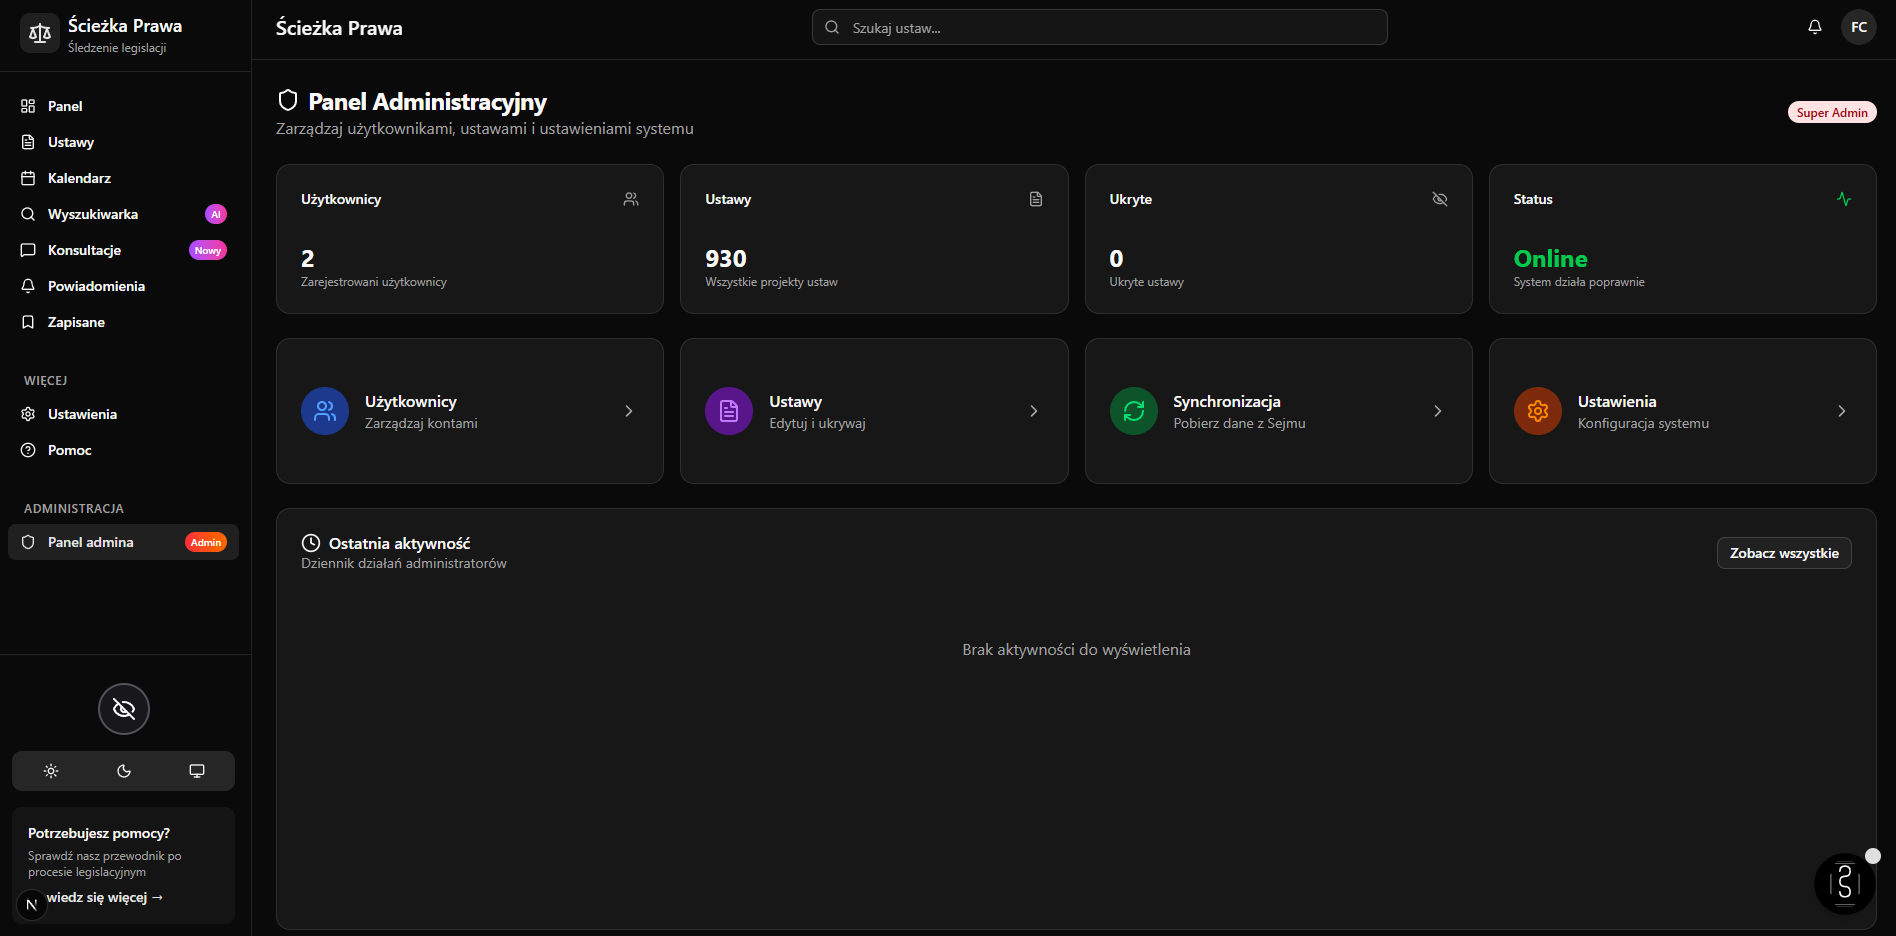
\includegraphics[width=\textwidth]{admin.png}
  \caption{Panel administracyjny z zarządzaniem użytkownikami, synchronizacją i logami}
  \label{fig:admin}
\end{figure}

% =============================================================================
% SEKCJA 8: STRONY I FUNKCJONALNOŚCI
% =============================================================================
\section{Strony i kluczowe funkcjonalności}

\subsection{Strona główna (Landing Page)}

Strona powitalna prezentująca funkcjonalności platformy z interaktywnym demo.

\textbf{Elementy:}
\begin{itemize}[leftmargin=2em]
  \item Banner z informacją o transmisji na żywo Sejmu
  \item Nagłówek Hero z gradientem i CTA
  \item Interaktywny mockup dashboardu z prawdziwymi danymi (20 projektów)
  \item Siatka 3 kluczowych funkcji (real-time, AI, powiadomienia)
  \item Statystyki (kadencja, posłowie, projekty/miesiąc, monitoring)
  \item Sekcja z formularzem rejestracji
\end{itemize}

\subsection{Panel główny (Dashboard)}

Centralny punkt aplikacji z przeglądem stanu legislacji.

\textbf{Elementy:}
\begin{itemize}[leftmargin=2em]
  \item 4 karty statystyk: łączna liczba projektów, aktywne, opublikowane, alerty
  \item Banner YouTube Live z auto-odświeżaniem co 2 minuty
  \item Tabela ostatnio zaktualizowanych projektów (5 newest)
  \item Rozkład statusów z paskami postępu
\end{itemize}

\subsection{Lista projektów ustaw}

Zaawansowane przeglądanie i filtrowanie projektów legislacyjnych.

\textbf{7 typów filtrów:} status, typ wnioskodawcy, kategoria, rok, kadencja, tagi, wyszukiwanie tekstowe.

\textbf{3 opcje sortowania:} ostatnia aktualizacja, data wpłynięcia, tytuł.

\textbf{Paginacja:} 10 projektów na stronę z nawigacją prev/next.

\subsection{Szczegóły projektu ustawy}

Kompleksowy widok z 8 zakładkami:

\begin{enumerate}[leftmargin=2em]
  \item \textbf{Ogólne} — opis, ministerstwo, daty, przycisk śledzenia
  \item \textbf{Ścieżka legislacyjna} — wizualizacja 11-etapowej osi czasu
  \item \textbf{Głosowania} — wyniki z podziałem na kluby parlamentarne
  \item \textbf{AI Pomoc} — 4 tryby analizy (prosty język, skutki, streszczenie, wyjaśnienie)
  \item \textbf{Ocena skutków} — wizualizacja danych OSR
  \item \textbf{Konsultacje} — forum komentarzy z wątkami i reakcjami
  \item \textbf{Propozycje} — system propozycji obywatelskich z głosowaniem
  \item \textbf{Ankiety} — tworzenie i przeglądanie wyników ankiet
\end{enumerate}

\begin{figure}[H]
  \centering
  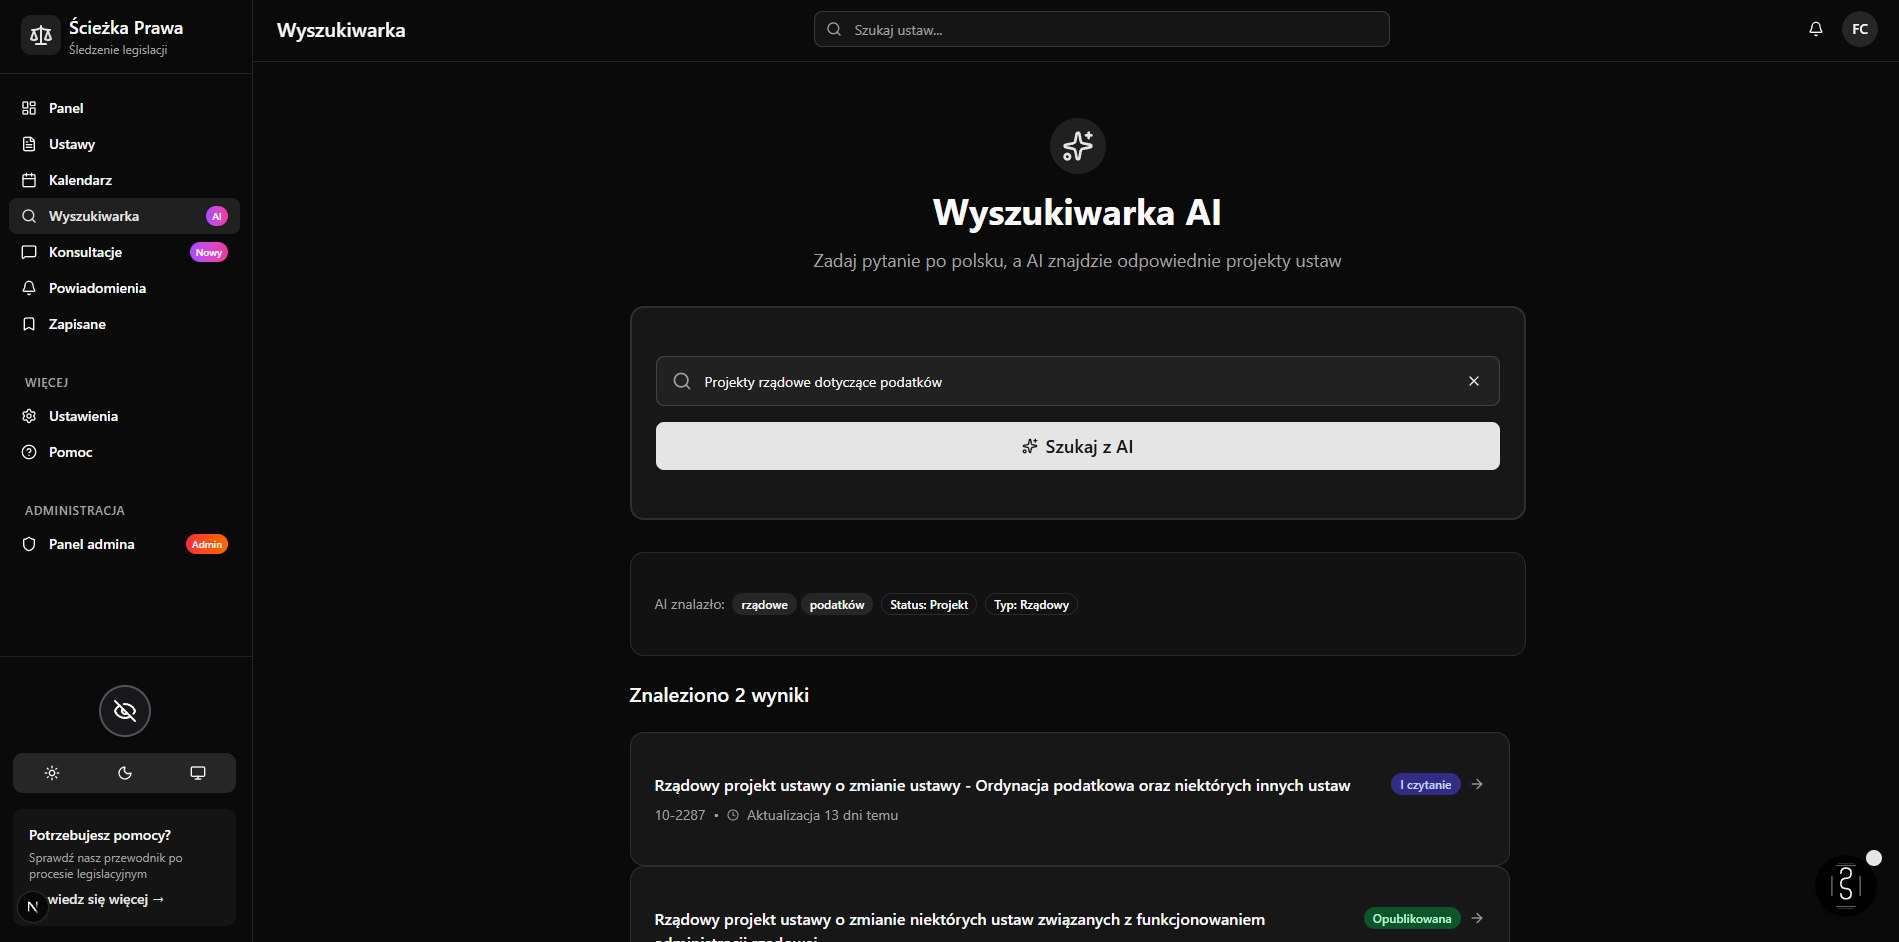
\includegraphics[width=\textwidth]{ai-search.png}
  \caption{Wyszukiwarka AI z analizą semantyczną zapytań i sugestiami filtrów}
  \label{fig:aisearch}
\end{figure}

\subsection{Wyszukiwarka AI}

Inteligentne wyszukiwanie projektów z analizą semantyczną:

\begin{itemize}[leftmargin=2em]
  \item Pole wyszukiwania z przetwarzaniem AI zapytania w języku naturalnym
  \item Automatyczne mapowanie na: kategorię, status, typ wnioskodawcy, ministerstwo
  \item Zapisywanie wyszukiwań na profilu użytkownika
  \item Wyniki z kartami statusu i metadanymi
\end{itemize}

\subsection{Kalendarz legislacyjny}

\begin{itemize}[leftmargin=2em]
  \item Widok miesiąca z kolorowanymi komórkami zdarzeń
  \item Kolory: Sejm (czerwony), Senat (niebieski), Komisje (fioletowy)
  \item Panel szczegółów wybranego dnia
  \item Lista nadchodzących zdarzeń (7 dni)
  \item Banner YouTube Live na górze strony
  \item Przełącznik widoku: miesiąc / lista
\end{itemize}

\subsection{Konsultacje publiczne}

\begin{figure}[H]
  \centering
  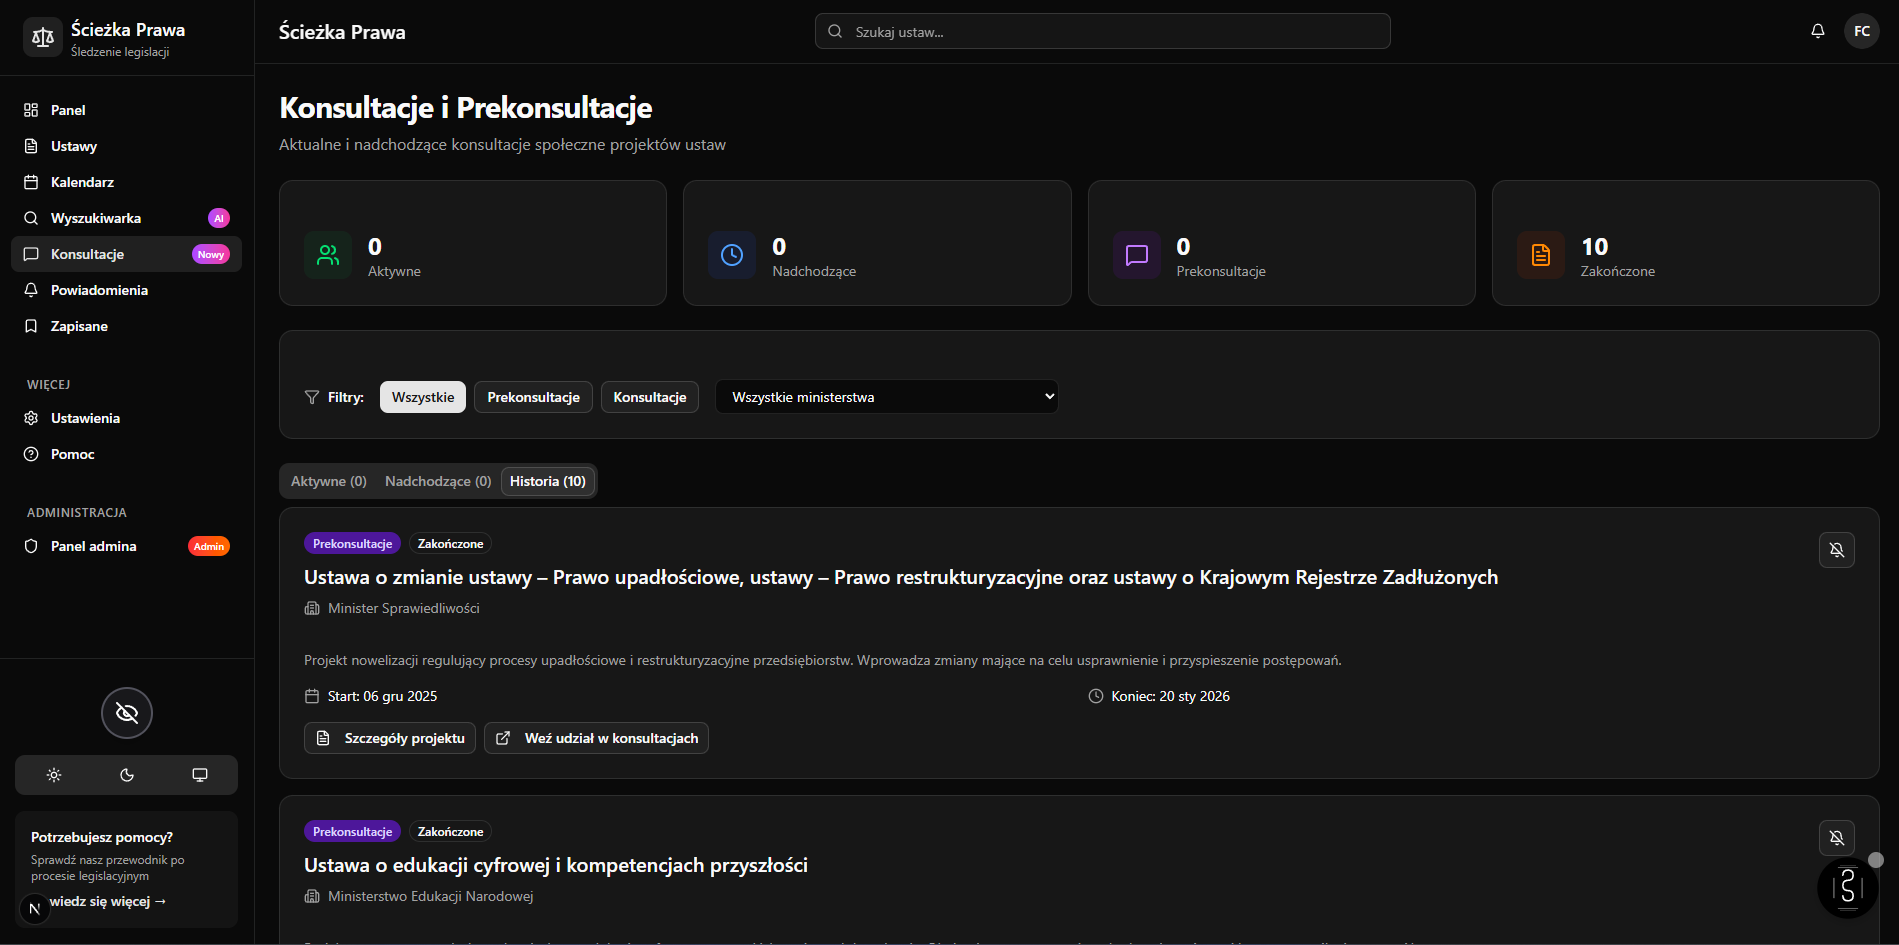
\includegraphics[width=\textwidth]{consultations.png}
  \caption{Strona konsultacji publicznych z aktywnymi i nadchodzącymi konsultacjami}
  \label{fig:consultations}
\end{figure}

\begin{itemize}[leftmargin=2em]
  \item 3 zakładki: Aktywne, Nadchodzące, Zakończone
  \item Filtrowanie po ministerstwie i typie (prekonsultacja/konsultacja)
  \item Karty z datami trwania, liczbą komentarzy i linkami
  \item 4 karty statystyk: aktywne, nadchodzące, prekonsultacje, zakończone
  \item Integracja z systemem RCL (Rządowe Centrum Legislacji)
\end{itemize}

\subsection{Panel administracyjny}

Panel dostępny dla użytkowników z rolą \texttt{moderator+}:

\begin{table}[H]
\centering
\renewcommand{\arraystretch}{1.3}
\begin{tabularx}{\textwidth}{l X}
\toprule
\textbf{Podstrona} & \textbf{Funkcjonalność} \\
\midrule
/admin & Dashboard z 4 statystykami, szybkie akcje, ostatnia aktywność \\
/admin/users & Zarządzanie rolami, blokowanie, wyszukiwanie użytkowników \\
/admin/bills & Edycja, ukrywanie/odkrywanie projektów \\
/admin/sync & Ręczna synchronizacja z API Sejmu i RCL \\
/admin/settings & 4 ustawienia: auto-sync, interwał, maintenance, rejestracja \\
/admin/logs & Dziennik aktywności administracyjnej z filtrami \\
/admin/test-notification & Testowanie systemu email \\
\bottomrule
\end{tabularx}
\caption{Podstrony panelu administracyjnego}
\end{table}

\newpage

% =============================================================================
% SEKCJA 9: DOSTĘPNOŚĆ I UX
% =============================================================================
\section{Dostępność (WCAG) i UX}

\subsection{Tryby dostępności}

Aplikacja implementuje zaawansowany system dostępności oparty na \texttt{AccessibilityProvider}:

\begin{table}[H]
\centering
\renewcommand{\arraystretch}{1.3}
\begin{tabularx}{\textwidth}{l X}
\toprule
\textbf{Funkcja} & \textbf{Opis} \\
\midrule
Tryb wysokiego kontrastu (jasny) & Czarny tekst na białym tle, żółte fokusowe obwódki \\
Tryb wysokiego kontrastu (ciemny) & Biały tekst na czarnym tle, wzmocnione kolory \\
Tryb odwróconego kontrastu & Inwersja kolorów dla specyficznych potrzeb \\
Regulacja rozmiaru czcionki & Suwak od 80\% do 200\% podstawowego rozmiaru \\
Nawigacja klawiaturą & Pełna obsługa Tab, Enter, Escape, klawisze strzałek \\
Ciemny/jasny motyw & Automatyczny na podstawie preferencji systemu \\
Panel dostępności & Sidebar z szybkim dostępem do wszystkich opcji \\
\bottomrule
\end{tabularx}
\caption{Funkcje dostępności WCAG}
\end{table}

\subsection{Responsywność}

\begin{itemize}[leftmargin=2em]
  \item Desktop: pełny sidebar + treść główna
  \item Tablet: zwijany sidebar z przyciskiem hamburger
  \item Mobilne: drawer navigation + uproszczony layout
  \item Wszystkie tabele i karty adaptują się do rozmiaru ekranu
\end{itemize}

\subsection{Język interfejsu}

Cały interfejs jest w~\textbf{języku polskim}:
\begin{itemize}[leftmargin=2em]
  \item Etykiety statusów: \textit{Opublikowana}, \textit{Senat}, \textit{Komisja}, \textit{I/II/III Czytanie}
  \item Formatowanie dat: \texttt{date-fns} z lokalizacją \texttt{\{locale: pl\}}
  \item Polskie komunikaty błędów, instrukcje i opisy
  \item Strony polityk: regulamin, prywatność, dostępność, cookies 
\end{itemize}

\newpage

% =============================================================================
% SEKCJA 10: ŚCIEŻKA LEGISLACYJNA
% =============================================================================
\section{Wizualizacja ścieżki legislacyjnej}

Jeden z kluczowych komponentów aplikacji — interaktywna oś czasu procesu legislacyjnego.

\subsection{13 statusów projektu ustawy}

\begin{figure}[H]
\centering
\begin{tikzpicture}[
  stage/.style={draw, rounded corners=3pt, minimum width=2.2cm, minimum height=0.7cm, 
                font=\tiny\bfseries, text centered, line width=0.4pt},
  arrow/.style={-{Stealth[length=4pt]}, thick, color=gray!50},
  scale=0.95
]
  % Preparatory row
  \node[stage, fill=hackgold!20, draw=hackgold!50] (cc) at (0, 2) {Współtworzenie};
  \node[stage, fill=hackgold!15, draw=hackgold!40] (pc) at (3, 2) {Prekonsultacja};
  \node[stage, fill=primaryblue!10, draw=primaryblue!30] (con) at (6, 2) {Konsultacje};
  \node[stage, fill=primaryblue!15, draw=primaryblue!40] (dr) at (9, 2) {Projekt};
  
  % Main process row
  \node[stage, fill=primaryblue!20, draw=primaryblue!50] (sub) at (0, 0) {Wpłynięcie};
  \node[stage, fill=primaryblue!25, draw=primaryblue!60] (r1) at (2.5, 0) {I Czytanie};
  \node[stage, fill=accentpurple!20, draw=accentpurple!50] (com) at (5, 0) {Komisja};
  \node[stage, fill=primaryblue!25, draw=primaryblue!60] (r2) at (7.5, 0) {II Czytanie};
  \node[stage, fill=primaryblue!30, draw=primaryblue!70] (r3) at (10, 0) {III Czytanie};
  
  % Final row
  \node[stage, fill=accentgreen!15, draw=accentgreen!40] (sen) at (2.5, -2) {Senat};
  \node[stage, fill=hackgold!25, draw=hackgold!60] (pres) at (5.5, -2) {Prezydent};
  \node[stage, fill=accentgreen!30, draw=accentgreen!70] (pub) at (8.5, -2) {Publikacja};
  
  % Rejected
  \node[stage, fill=accentred!15, draw=accentred!50] (rej) at (12, 0) {Odrzucona};
  
  % Arrows
  \draw[arrow] (cc) -- (pc);
  \draw[arrow] (pc) -- (con);
  \draw[arrow] (con) -- (dr);
  \draw[arrow] (dr) -- (sub);
  \draw[arrow] (sub) -- (r1);
  \draw[arrow] (r1) -- (com);
  \draw[arrow] (com) -- (r2);
  \draw[arrow] (r2) -- (r3);
  \draw[arrow] (r3) -- (sen);
  \draw[arrow] (sen) -- (pres);
  \draw[arrow] (pres) -- (pub);
  
  % Rejection arrows
  \draw[arrow, dashed, color=accentred!50] (r1) -- (rej);
  \draw[arrow, dashed, color=accentred!50] (r3) -- (rej);
  
  % Labels
  \node[above=0.3cm of pc, font=\scriptsize\color{gray}] {Etapy przygotowawcze (opcjonalne)};
  \node[below=0.3cm of com, font=\scriptsize\color{gray}] {Proces parlamentarny};
\end{tikzpicture}
\caption{Pełna ścieżka legislacyjna z 13 możliwymi statusami}
\label{fig:legislative}
\end{figure}

\subsection{Etapy w szczegółach}

\begin{longtable}{>{\bfseries}l l p{8cm}}
\toprule
\textbf{Status} & \textbf{Klucz} & \textbf{Opis} \\
\midrule
\endhead
Współtworzenie & co\_creation & Wczesna faza partycypacji obywatelskiej \\
Prekonsultacja & preconsultation & Wstępne konsultacje przed formalizacją \\
Konsultacje & consultation & Oficjalne konsultacje publiczne (RCL) \\
Projekt & draft & Formalny projekt ustawy \\
Wpłynięcie & submitted & Złożenie projektu w Sejmie \\
I Czytanie & first\_reading & Pierwsze czytanie w Sejmie \\
Komisja & committee & Prace komisji sejmowej \\
II Czytanie & second\_reading & Drugie czytanie \\
III Czytanie & third\_reading & Trzecie czytanie i głosowanie \\
Senat & senate & Rozpatrzenie przez Senat \\
Prezydent & presidential & Oczekiwanie na podpis Prezydenta \\
Opublikowana & published & Ustawa w mocy (Dz.U., ELI) \\
Odrzucona & rejected & Projekt odrzucony (na dowolnym etapie) \\
\bottomrule
\caption{Szczegółowy opis 13 statusów legislacyjnych}
\end{longtable}

\newpage

% =============================================================================
% SEKCJA 11: AI I BAZA WIEDZY
% =============================================================================
\section{System AI i baza wiedzy}

\subsection{Architektura AI}

System AI oparty jest na trzech filarach:

\begin{enumerate}[leftmargin=2em]
  \item \textbf{Google Gemini 2.0 Flash} — główny model do analizy tekstu prawnego
  \item \textbf{Lokalna baza wiedzy (RAG)} — \texttt{src/lib/ai/knowledge-base.ts} z wiedzą o procesie legislacyjnym
  \item \textbf{Cachowanie localStorage} — 24-godzinny cache odpowiedzi AI po stronie klienta
\end{enumerate}

\subsection{4 tryby analizy tekstu}

\begin{table}[H]
\centering
\renewcommand{\arraystretch}{1.4}
\begin{tabularx}{\textwidth}{l l X}
\toprule
\textbf{Tryb} & \textbf{Nazwa PL} & \textbf{Opis działania} \\
\midrule
simple & Prosty Język & Przepisuje tekst prawny językiem zrozumiałym dla laika. Używa prostych słów i krótkich zdań. \\
impact & Analiza Skutków & Analizuje wpływ na: obywateli, firmy, budżet, środowisko. Podaje daty wejścia w życie i kontrowersje. \\
summary & Streszczenie & Generuje kompaktowe podsumowanie w 3-5 zdaniach z kluczowymi punktami. \\
explain & Wyjaśnienie & Szczegółowe definicje terminów prawnych z emoji nagłówkami i przykładami. \\
\bottomrule
\end{tabularx}
\caption{4 tryby analizy AI dostępne dla każdego projektu ustawy}
\end{table}

\subsection{Asystent konwersacyjny}

Komponent \texttt{AIAssistant} — chatbot z bazą wiedzy:

\begin{itemize}[leftmargin=2em]
  \item Priorytetowo: wyszukiwanie w lokalnej bazie wiedzy (RAG)
  \item Fallback: Google Gemini API gdy brak odpowiedzi w bazie
  \item Graceful degradation: działa bez klucza API (tylko baza lokalna)
  \item Kontekst: opisy funkcji aplikacji, etapy legislacyjne, FAQ
\end{itemize}

\subsection{Baza wiedzy RAG}

Plik \texttt{src/lib/ai/knowledge-base.ts} zawiera:

\begin{itemize}[leftmargin=2em]
  \item Opisy funkcji aplikacji (10 sekcji)
  \item Definicje 10 etapów procesu legislacyjnego
  \item Wyjaśnienia ról parlamentarnych
  \item Opisy typów wnioskodawców
  \item 8 najczęstszych pytań (FAQ)
\end{itemize}

\newpage

% =============================================================================
% SEKCJA 12: KOMPONENTY UI
% =============================================================================
\section{Komponenty interfejsu użytkownika}

\subsection{Biblioteka komponentów ShadCN/Radix}

Aplikacja korzysta z 26 komponentów ShadCN UI opartych na Radix Primitives:

\begin{table}[H]
\centering
\renewcommand{\arraystretch}{1.2}
\footnotesize
\begin{tabularx}{\textwidth}{X X X X}
\toprule
\textbf{Komponent} & \textbf{Komponent} & \textbf{Komponent} & \textbf{Komponent} \\
\midrule
Accordion & Alert & Avatar & Badge \\
Button & Card & Checkbox & Collapsible \\
Dialog & Dropdown Menu & Input & Label \\
Pagination & Popover & Progress & Radio Group \\
Scroll Area & Select & Separator & Sheet \\
Skeleton & Slider & Switch & Tabs \\
Textarea & Tooltip & & \\
\bottomrule
\end{tabularx}
\caption{26 komponentów ShadCN UI w projekcie}
\end{table}

\subsection{Komponenty domenowe — projekty ustaw}

\begin{table}[H]
\centering
\renewcommand{\arraystretch}{1.3}
\footnotesize
\begin{tabularx}{\textwidth}{l X}
\toprule
\textbf{Komponent} & \textbf{Opis} \\
\midrule
AlertButton & Przycisk subskrypcji zmian w projekcie \\
LegislativeTimeline & Wizualna oś czasu z 11 etapami i kolorami statusu \\
LegislativeTrainEnhanced & Rozszerzona wizualizacja w stylu EU-train \\
SimpleLanguageHelper & AI translator z 4 zakładkami trybów \\
ImpactAssessmentViewer & Wizualizacja wyników OSR (Ocena Skutków Regulacji) \\
ImpactAssessmentEnhanced & Rozszerzona wersja z wykresami \\
ConsultationForum & Forum wątków komentarzy z reakcjami \\
ProposalList & Lista propozycji obywatelskich z głosowaniem \\
VotingPieChart & Wykres wyników głosowań z podziałem na kluby \\
SurveyViewer & Przeglądanie i wypełnianie ankiet \\
\bottomrule
\end{tabularx}
\caption{Kluczowe komponenty domenowe dla projektów ustaw}
\end{table}

\subsection{Layout i nawigacja}

\begin{itemize}[leftmargin=2em]
  \item \textbf{DashboardLayout} — główny wrapper z sidebar i headerem
  \item \textbf{Sidebar} — nawigacja z elementami zależnymi od roli (admin = dodatkowe opcje)
  \item \textbf{Header} — pasek wyszukiwania, powiadomienia, menu użytkownika
  \item \textbf{MobileNav} — drawer nawigacyjny na urządzeniach mobilnych
  \item \textbf{AccessibilityButton} — przycisk szybkiego dostępu do panelu dostępności
\end{itemize}

\newpage

% =============================================================================
% SEKCJA 13: KONFIGURACJA I WDROŻENIE
% =============================================================================
\section{Konfiguracja i wdrożenie}

\subsection{Zmienne środowiskowe}

\begin{table}[H]
\centering
\renewcommand{\arraystretch}{1.3}
\begin{tabularx}{\textwidth}{l l X}
\toprule
\textbf{Zmienna} & \textbf{Wymagana} & \textbf{Opis} \\
\midrule
NEXT\_PUBLIC\_SUPABASE\_URL & Tak & URL instancji Supabase \\
NEXT\_PUBLIC\_SUPABASE\_ANON\_KEY & Tak & Klucz anonimowy (publiczny) \\
SUPABASE\_SERVICE\_ROLE\_KEY & Tak & Klucz serwisowy (omija RLS) \\
GEMINI\_API\_KEY & Nie* & Klucz Google Gemini 2.0 Flash \\
RESEND\_API\_KEY & Nie* & Klucz Resend do emaili \\
\bottomrule
\end{tabularx}
\caption{Zmienne środowiskowe (* — opcjonalne, aplikacja działa bez nich z ograniczoną funkcjonalnością)}
\end{table}

\subsection{Komendy deweloperskie}

\begin{lstlisting}[style=typescript, title=Komendy package.json]
npm run dev          # Start z Turbopack (port 3000)
npm run build        # Build produkcyjny
npm run start        # Start serwera produkcyjnego
npm run lint         # ESLint
\end{lstlisting}

\subsection{Konfiguracja Next.js}

\begin{lstlisting}[style=typescript, title=next.config.ts]
const nextConfig = {
  // App Router (domyslny w Next.js 16)
  // Turbopack dev server
  // TypeScript strict mode
  // Tailwind CSS 4 integration
}
\end{lstlisting}

\subsection{Konfiguracja TypeScript}

\begin{lstlisting}[style=typescript, title=tsconfig.json (kluczowe opcje)]
{
  "compilerOptions": {
    "target": "ES2017",
    "lib": ["dom", "dom.iterable", "esnext"],
    "strict": true,
    "jsx": "react-jsx",
    "moduleResolution": "bundler",
    "paths": { "@/*": ["./src/*"] }
  }
}
\end{lstlisting}

\subsection{Wdrożenie produkcyjne}

Rekomendowane platformy wdrożeniowe:

\begin{enumerate}[leftmargin=2em]
  \item \textbf{Vercel} — natywne wsparcie Next.js, automatyczne deployments z Git
  \item \textbf{Supabase Cloud} — zarządzana baza danych PostgreSQL z RLS
  \item \textbf{Resend} — darmowy plan 100 emaili/dzień
  \item \textbf{Google AI Studio} — darmowy tier Gemini 2.0 Flash
\end{enumerate}

\newpage

% =============================================================================
% SEKCJA 14: PODSUMOWANIE
% =============================================================================
\section{Podsumowanie}

\subsection{Statystyki projektu}

\begin{table}[H]
\centering
\renewcommand{\arraystretch}{1.4}
\begin{tabularx}{\textwidth}{l X}
\toprule
\textbf{Metryka} & \textbf{Wartość} \\
\midrule
Endpointy API & 34 route handlers \\
Tabele bazy danych & 8 głównych + typy ENUM \\
Komponenty UI (ShadCN) & 26 \\
Komponenty domenowe & 15+ \\
Strony aplikacji & 18 (publiczne + auth + admin) \\
Statusy legislacyjne & 13 \\
Tryby AI & 6 (4 analiza + chat + search) \\
Role użytkowników & 4 (hierarchiczne) \\
Polityki RLS & Włączone na wszystkich tabelach \\
Integracje API & 4 (Sejm, YouTube, Gemini, Resend) \\
Tryby dostępności & 4 (kontrast jasny/ciemny/odwrócony + rozmiar) \\
\bottomrule
\end{tabularx}
\caption{Podsumowanie statystyk projektu}
\end{table}

\subsection{Kluczowe osiągnięcia}

\begin{itemize}[leftmargin=2em]
  \item \textbf{Pełna automatyzacja} synchronizacji danych z oficjalnego API Sejmu RP
  \item \textbf{Analiza AI} tekstu prawnego z 4 różnymi trybami w czasie rzeczywistym
  \item \textbf{System partycypacji obywatelskiej} — konsultacje, propozycje, ankiety
  \item \textbf{Kompleksowe bezpieczeństwo} — RLS, hierarchia ról, logowanie admina
  \item \textbf{Pełna dostępność WCAG} — tryby kontrastu, regulacja rozmiaru, nawigacja klawiaturą
  \item \textbf{Responsywny design} od desktopa po urządzenia mobilne
  \item \textbf{DX (Developer Experience)} — TypeScript strict, ESLint, komponenty ShadCN
\end{itemize}

\vspace{1.5cm}

\begin{center}
\begin{tikzpicture}
  \node[draw=hackgold, fill=hackgold!8, rounded corners=10pt, line width=2pt, 
        inner sep=20pt, text width=12cm, text centered] {
    {\Large\bfseries\textcolor{hackgold!80!black}{Ścieżka Prawa}}\\[8pt]
    {\large\textcolor{gray}{Zwycięski Projekt HackNation PL 2025}}\\[12pt]
    {\textcolor{gray}{Autor: \textbf{Filip Czerwiński}}}\\[4pt]
    {\textcolor{gray}{Stos: Next.js 16 · React 19 · Supabase · Gemini 2.0 Flash}}\\[4pt]
    {\small\textcolor{gray!70}{Przejrzystość prawa w Twoich rękach.}}
  };
\end{tikzpicture}
\end{center}

\end{document}
